\documentclass[11pt]{article}
\usepackage[a4paper,margin=2.5cm]{geometry}
\usepackage{booktabs}
\usepackage{graphicx}
\usepackage{subcaption}
\usepackage{amsmath}
\usepackage{float}
\usepackage{adjustbox}
\usepackage[hidelinks]{hyperref}
\graphicspath{{../../results/task3/plots/}}
\setlength{\parskip}{0.6em}
\setlength{\parindent}{0pt}

\begin{document}
\setcounter{section}{2}

\section{Task 3: Incorporating SPP with Dynamic I-RRIP}

\subsection{Goal}

Task 3 runs the Stride Pattern Prefetcher (SPP) from Task 1B at the L1D together with the
Dynamic I-RRIP L2 policy from Task 2B. The L2 replacement policy is then made \emph{aware} of
the lines that SPP brings in, which it can recognise by the packet type \texttt{PREFETCH}. The
target is a higher IPC than both standalone SPP and Dynamic I-RRIP.

The two mechanisms attack different misses. SPP is a data prefetcher: it removes L1D data misses
and does nothing for instructions. Dynamic I-RRIP removes L2 instruction misses and pays for it
with extra L2 data misses. The prefetch-aware part decides how the L2 should treat the extra,
speculative lines that SPP adds to the L2 traffic.

\subsection{Experimental setup}

The setup is the same as in Tasks 1B and 2B: ChampSim, 1 core, hashed perceptron branch
predictor, 48~KiB 12-way L1D, 512~KiB 8-way L2, 2~MiB 16-way LLC, 25M warm-up followed by 25M
measured instructions on the three provided traces. All binaries were built and run with
\texttt{gcc 7.5}. The only prefetcher is the L1D prefetcher. We evaluate five configurations:

\begin{itemize}
  \item \textbf{Baseline:} no prefetcher, LRU at the L2. This is the reference for speedup and
        coverage, as in Task 1B.
  \item \textbf{Dynamic I-RRIP:} no prefetcher, the Task 2B policy at the L2 ($T=0.05$).
  \item \textbf{SPP + LRU:} standalone SPP (\texttt{prefetcher/spp.l1d\_pref}, unchanged from
        Task 1B).
  \item \textbf{SPP + Dyn I-RRIP (unaware):} SPP with the Task 2B policy, which treats prefetched
        lines like any other data line. This is the same binary as the next configuration, run
        with \texttt{DYN\_IRRIP\_PF\_AWARE=0}.
  \item \textbf{SPP + PF-aware Dyn I-RRIP:} this task, \texttt{replacement/dyn\_irrip.l2c\_repl}.
\end{itemize}

All five configurations were re-run on the current code base (with the Task 2 changes merged), so
that they can be compared like for like. The baseline IPCs are identical to those of Tasks 1B and
2B. Our SPP + LRU speedups (1.0087, 1.0065, 1.0160) are within 0.25\% of the Task 1B report.

\textbf{Metrics.} IPC is the cumulative IPC of the measured region, and
$\text{Speedup} = \text{IPC} / \text{IPC}_{\text{baseline}}$. Prefetch accuracy is ChampSim's L1D
statistic, \emph{useful load prefetches / prefetches issued to the lower level}, as in Task 1B.
Coverage is
\[
\text{Coverage} = \frac{\text{L1D load misses}_{\text{baseline}} - \text{L1D load misses}}
{\text{L1D load misses}_{\text{baseline}}}.
\]
L1D and L2C load MPKI are taken from ChampSim's
statistics, and the L2 load MPKI is split into instruction and data loads as in Task 2. Averages
use the geometric mean for IPC and speedup and the arithmetic mean for everything else.

\subsection{How SPP's prefetches reach the L2}
\label{sec:traffic}

Before designing the policy, we measured what the L2 actually sees from SPP
(Table~\ref{tab:traffic}).

\begin{table}[H]
\centering
\small
\setlength{\tabcolsep}{4pt}
\begin{adjustbox}{max width=\textwidth}
\begin{tabular}{llrrrrrr}
\toprule
Trace & L2 policy & SPP prefetch & Sent to & L2 prefetch & L2 prefetch & Prefetched lines & LLC load \\
 & & requests & the L2 & hits (rate) & fills & demand-hit in L2 & misses \\
\midrule
Trace1 & LRU & 777\,706 & 64\,650 & 17\,493 (27.6\%) & 45\,833 & -- & 293\,113 \\
 & Dyn (unaware) & 778\,996 & 64\,781 & 5\,026 (7.9\%) & 58\,397 & 1\,013 (1.7\%) & 277\,907 \\
 & Dyn (PF-aware) & 779\,929 & 64\,706 & 5\,006 (7.9\%) & 58\,364 & 981 (1.7\%) & 277\,422 \\
\midrule
Trace2 & LRU & 522\,717 & 27\,901 & 7\,331 (26.4\%) & 20\,391 & -- & 196\,869 \\
 & Dyn (unaware) & 516\,212 & 27\,811 & 2\,461 (8.9\%) & 25\,137 & 490 (1.9\%) & 199\,386 \\
 & Dyn (PF-aware) & 514\,884 & 27\,630 & 2\,437 (8.9\%) & 24\,951 & 529 (2.1\%) & 199\,287 \\
\midrule
Trace3 & LRU & 827\,440 & 34\,024 & 2\,890 (8.6\%) & 30\,583 & -- & 63\,285 \\
 & Dyn (unaware) & 826\,212 & 33\,975 & 1\,017 (3.0\%) & 32\,426 & 382 (1.2\%) & 58\,942 \\
 & Dyn (PF-aware) & 825\,041 & 33\,887 & 1\,003 (3.0\%) & 32\,310 & 388 (1.2\%) & 58\,886 \\
\bottomrule
\end{tabular}
\end{adjustbox}
\caption{SPP's traffic at the L2 over the 25M measured instructions. ``Sent to the L2'' is
ChampSim's \emph{prefetches issued to lower level}. ``Prefetched lines demand-hit in L2'' counts
prefetch fills that later served a demand access in the L2, out of all prefetch fills. It is
measured by the policy's statistics, which LRU does not have.}
\label{tab:traffic}
\end{table}

Three observations shaped the design:
\begin{enumerate}
  \item \textbf{The L2 sees little prefetch traffic.} More than 90\% of SPP's requests never leave the
        L1D, because the line is already there or the request is merged. Only 1.1--2.6 prefetches per kilo-instruction reach the L2,
        compared with 24, 53 and 4.9 L2 demand loads per kilo-instruction on Trace1--3. Any
        prefetch-specific rule can therefore move IPC only a little.
  \item \textbf{The L2 copy of a prefetched line is rarely used by a demand access.} Almost all
        prefetches are \texttt{FILL\_L1}: 27\,274 of 27\,901 on Trace2 have the same fill and
        origin level. The line is placed in the L1D as well, and the L1D serves the demand access.
        Only 1.2--2.1\% of prefetch fills ever get a demand hit in the L2. The rest are evicted
        unused, or are still resident at the end of the run.
  \item \textbf{Dynamic I-RRIP lowers the L2 hit rate of prefetch requests} from 26--28\% (LRU)
        to 8--9\% on Trace1 and Trace2. Its strict instruction mode evicts data first, so the
        lines that SPP asks for again are more often gone. Each such miss becomes an LLC access,
        which makes the prefetch later.
\end{enumerate}

\subsection{Design: handling the prefetch packet}

The prefetch awareness consists of three rules in \texttt{l2c\_update\_replacement\_state}, all
keyed on \texttt{type == PREFETCH}. Every other packet type is handled exactly as in Task 2B.
With no prefetcher, the policy is therefore identical to Task 2B: the no-prefetch runs reproduce
the Task 2B results cycle for cycle (Trace1: 106\,568\,235 cycles in both runs; likewise on Trace2 and Trace3).

\begin{table}[H]
\centering
\small
\begin{adjustbox}{max width=\textwidth}
\begin{tabular}{lll}
\toprule
Event & Task 2B (unaware) & Task 3 (prefetch-aware) \\
\midrule
Prefetch request in a leader set & not counted & not counted (unchanged) \\
Prefetch fill (miss), any set, any mode & RRPV 2 (as demand data) & \textbf{RRPV 1} \\
Prefetch request hits in the L2 & normal promotion & normal promotion (kept) \\
Demand hit on a prefetched line & normal promotion & normal promotion \\
Eviction & strict data-first / SRRIP & unchanged; prefetched lines are data \\
\bottomrule
\end{tabular}
\end{adjustbox}
\caption{Treatment of prefetched lines. The RRPV ordering in instruction mode becomes
\emph{code (0) $<$ prefetched data (1) $<$ demand data (2)}. In SRRIP mode and in the leader
sets, prefetched lines are inserted one step further from eviction than demand fills. In both, lower RRPV means
kept longer.}
\label{tab:design}
\end{table}

\paragraph{Rule 1: prefetches never enter the set-dueling decision.} The leader-set counters
count only demand accesses (loads, RFOs, translations). Prefetches are speculative, they are
always data, and their number depends on how aggressive SPP currently is, not on what the core is
waiting for. Counting them would lower the instruction share $r$ whenever SPP is aggressive, and
could switch off instruction priority for the wrong reason. Task 2B already filtered prefetches
out of the counters, but without a prefetcher the rule never applied; with SPP it is what keeps
the mode decision correct. With SPP running, the leaders still measure $r \approx 0.42$--$0.45$,
$0.66$ and $0.17$ on Trace1--3, similar to the values without a prefetcher in Task 2B.

\paragraph{Rule 2: a prefetch fill is inserted at RRPV 1.} This value is a compromise between two
facts from Section~\ref{sec:traffic}.
\begin{itemize}
  \item \emph{Do not pin prefetched lines.} Their L2 copy rarely serves a demand access, because
        the L1D holds its own copy. When we shielded unused prefetched lines from eviction while
        other data was present, the speedup fell from 1.0301 to 1.0235 (Table~\ref{tab:explore}), and LLC load misses rose
        (Trace1: 284\,727 instead of 277\,422). The extra resident prefetches pushed out demand data that was
        about to be reused.
  \item \emph{Do not throw them away either.} Inserting them at RRPV~3 (``dead on arrival'')
        lowers the speedup to 1.0284 and raises LLC load misses on every trace. For example, on
        Trace1 it is 279\,727 compared with 277\,422. A prefetched line is still a predicted
        future demand access: SPP's L1D accuracy is 38--53\%. The L1D (48~KiB) may drop the line
        before it is used, and SPP regularly requests the same lines again (the L2 prefetch hits
        in Table~\ref{tab:traffic}). About 2\% of the prefetches have a different fill level
        (\texttt{FILL\_L2}, issued when the L1D MSHR is more than half full), and for those the L2 copy
        is the only copy. The
        replacement interface receives only the packet type, so these cannot be told apart from
        \texttt{FILL\_L1} prefetches, and a single mild level of protection is used for all.
\end{itemize}
RRPV~1 places a prefetched line just above demand-fetched data but below code. A demand-fetched
data line has already delivered its first use to the L1D, whereas a prefetched line has not been
used yet. It keeps the strict instruction priority of Task 2B intact: code is still never
evicted while any data line is present. The sensitivity study in Section~\ref{sec:sens} shows
that RRPV~1 is the best of the four possible values, although RRPV~0 is very close.

\paragraph{Rule 3: prefetch hits are promoted like data hits.} A prefetch request that hits in the
L2 means SPP has just predicted a demand access to that line, so it is treated like a data hit:
RRPV~0 in SRRIP mode and one step down in instruction mode. Leaving the RRPV unchanged on a
prefetch hit (as some prefetch-aware RRIP proposals do) was measured to be slightly worse
(Table~\ref{tab:explore}).

\paragraph{The prefetch rule applies in the leader sets too.} The leaders should measure the
system as it actually runs, prefetches included. If they ignored prefetches (plain SRRIP insertion),
the result was practically identical (1.0297 vs 1.0298 for the matching variants), so we keep one
uniform rule.

\paragraph{Hardware cost.} The type of the incoming request is already part of the request (MSHR
entry), so the prefetch awareness needs no new storage. It needs only a comparator on the type
field and a third insertion value. The total cost stays at the Task 2B figure of 50 bits on top
of I-RRIP. The \texttt{l2\_is\_pf} bit array in the code feeds only the statistics in
Table~\ref{tab:traffic}. It is not read by the policy and would not exist in hardware.

\subsection{Results}
\label{sec:results}

Table~\ref{tab:main} and Table~\ref{tab:mainl2} report all required metrics, and
Figures~\ref{fig:perf}--\ref{fig:l2} plot them. The raw values are in
\texttt{results/task3/task3\_results.csv}, the tables in \texttt{results/task3/task3\_tables.md},
and all logs in \texttt{results/task3/<configuration>/}.

\begin{table}[H]
\centering
\small
\begin{adjustbox}{max width=\textwidth}
\begin{tabular}{llrrrrr}
\toprule
Trace & Configuration & IPC & Speedup & Accuracy (\%) & Coverage (\%) & L1D load MPKI \\
\midrule
Trace1 & Baseline & 0.2322 & 1.0000 & -- & -- & 10.679 \\
 & Dyn I-RRIP & 0.2346 & 1.0101 & -- & -- & 10.680 \\
 & SPP + LRU & 0.2343 & 1.0087 & 53.09 & 9.63 & 9.650 \\
 & SPP + Dyn (unaware) & 0.2374 & 1.0222 & 52.93 & 9.53 & 9.661 \\
 & \textbf{SPP + PF-aware Dyn} & \textbf{0.2375} & \textbf{1.0226} & 52.86 & 9.53 & 9.662 \\
\midrule
Trace2 & Baseline & 0.2513 & 1.0000 & -- & -- & 13.536 \\
 & Dyn I-RRIP & 0.2601 & 1.0349 & -- & -- & 13.545 \\
 & SPP + LRU & 0.2529 & 1.0065 & 44.98 & 2.67 & 13.175 \\
 & SPP + Dyn (unaware) & 0.2621 & 1.0430 & 44.40 & 2.58 & 13.188 \\
 & \textbf{SPP + PF-aware Dyn} & \textbf{0.2625} & \textbf{1.0445} & 44.50 & 2.57 & 13.189 \\
\midrule
Trace3 & Baseline & 0.3819 & 1.0000 & -- & -- & 3.403 \\
 & Dyn I-RRIP & 0.3840 & 1.0057 & -- & -- & 3.404 \\
 & SPP + LRU & 0.3880 & 1.0160 & 37.94 & 13.85 & 2.932 \\
 & SPP + Dyn (unaware) & 0.3906 & 1.0229 & 37.85 & 13.76 & 2.935 \\
 & \textbf{SPP + PF-aware Dyn} & \textbf{0.3907} & \textbf{1.0232} & 37.97 & 13.78 & 2.934 \\
\midrule
Average & Baseline & 0.2814 & 1.0000 & -- & -- & 9.206 \\
 & Dyn I-RRIP & 0.2861 & 1.0168 & -- & -- & 9.210 \\
 & SPP + LRU & 0.2843 & 1.0104 & 45.34 & 8.72 & 8.586 \\
 & SPP + Dyn (unaware) & 0.2897 & 1.0293 & 45.06 & 8.62 & 8.595 \\
 & \textbf{SPP + PF-aware Dyn} & \textbf{0.2899} & \textbf{1.0301} & 45.11 & 8.63 & 8.595 \\
\bottomrule
\end{tabular}
\end{adjustbox}
\caption{IPC, speedup over the baseline, and the L1D prefetch metrics. Accuracy and coverage
exist only for the configurations with SPP.}
\label{tab:main}
\end{table}

\begin{table}[H]
\centering
\small
\begin{adjustbox}{max width=\textwidth}
\begin{tabular}{llrrrrr}
\toprule
Trace & Configuration & L2C load & L2 instr & L2 data & Avg.\ L2 miss & LLC load \\
 & & MPKI & load MPKI & load MPKI & latency (cyc.) & misses \\
\midrule
Trace1 & Baseline & 17.703 & 10.368 & 7.334 & 140.5 & 307\,044 \\
 & Dyn I-RRIP & 19.042 & 9.072 & 9.970 & 107.1 & 292\,496 \\
 & SPP + LRU & 16.825 & 10.392 & 6.434 & 141.9 & 293\,113 \\
 & SPP + Dyn (unaware) & 17.873 & 9.043 & 8.830 & 108.2 & 277\,907 \\
 & \textbf{SPP + PF-aware Dyn} & 17.878 & 9.044 & 8.834 & 108.2 & \textbf{277\,422} \\
\midrule
Trace2 & Baseline & 27.560 & 18.892 & 8.668 & 88.9 & 204\,533 \\
 & Dyn I-RRIP & 21.379 & 9.264 & 12.115 & 82.8 & 206\,936 \\
 & SPP + LRU & 27.486 & 19.132 & 8.354 & 89.4 & 196\,869 \\
 & SPP + Dyn (unaware) & 21.041 & 9.298 & 11.742 & 83.4 & 199\,386 \\
 & \textbf{SPP + PF-aware Dyn} & \textbf{20.844} & \textbf{9.096} & 11.748 & 83.7 & 199\,287 \\
\midrule
Trace3 & Baseline & 3.960 & 1.124 & 2.837 & 156.9 & 78\,933 \\
 & Dyn I-RRIP & 3.994 & 0.727 & 3.267 & 109.3 & 74\,944 \\
 & SPP + LRU & 3.313 & 1.144 & 2.169 & 158.3 & 63\,285 \\
 & SPP + Dyn (unaware) & 3.308 & 0.725 & 2.583 & 113.1 & 58\,942 \\
 & \textbf{SPP + PF-aware Dyn} & \textbf{3.307} & \textbf{0.723} & 2.585 & 113.1 & \textbf{58\,886} \\
\midrule
Average & Baseline & 16.408 & 10.128 & 6.280 & 128.8 & -- \\
 & Dyn I-RRIP & 14.805 & 6.354 & 8.451 & 99.7 & -- \\
 & SPP + LRU & 15.875 & 10.222 & 5.652 & 129.8 & -- \\
 & SPP + Dyn (unaware) & 14.074 & 6.356 & 7.718 & 101.6 & -- \\
 & \textbf{SPP + PF-aware Dyn} & \textbf{14.010} & \textbf{6.288} & 7.722 & 101.7 & -- \\
\bottomrule
\end{tabular}
\end{adjustbox}
\caption{L2 demand-load MPKI (total, instruction, data), with the average L2 miss latency and
the LLC demand-load misses (loads that went to DRAM) as supporting metrics.}
\label{tab:mainl2}
\end{table}

\begin{figure}[H]
\centering
\begin{subfigure}{0.49\textwidth}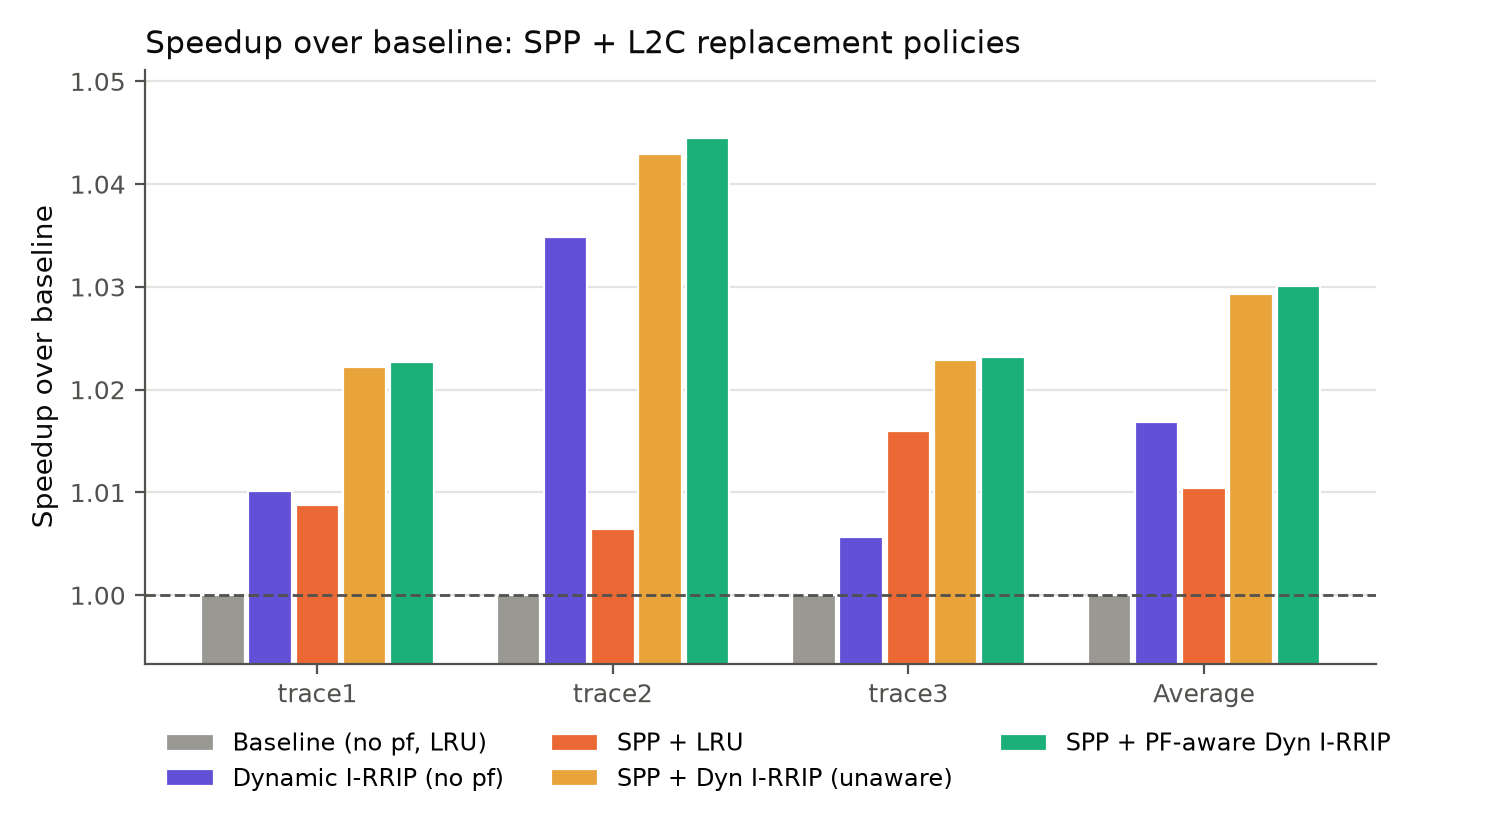
\includegraphics[width=\linewidth]{speedup.png}\caption{Speedup over the baseline.}\end{subfigure}
\begin{subfigure}{0.49\textwidth}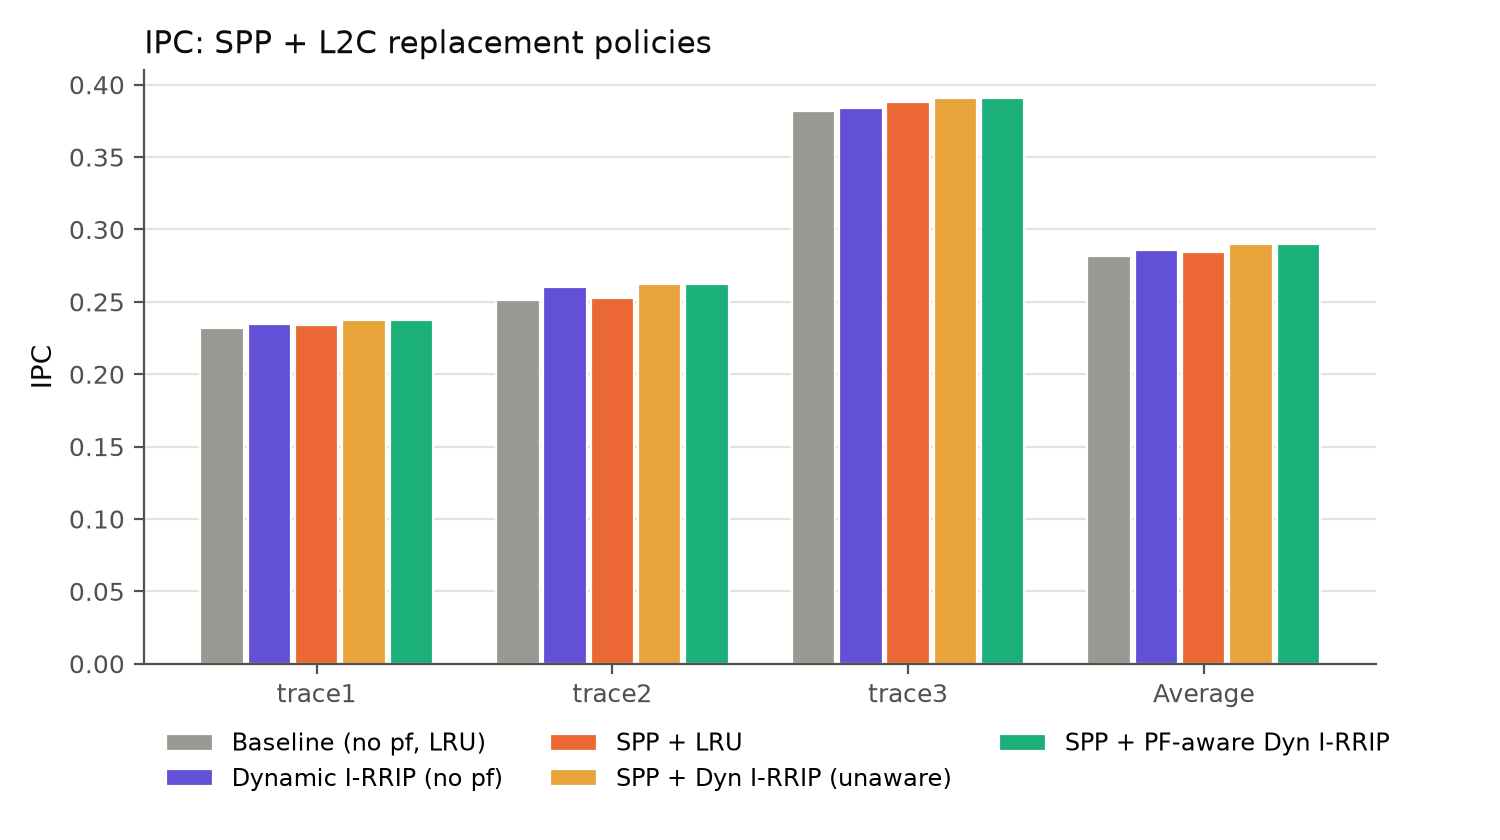
\includegraphics[width=\linewidth]{ipc.png}\caption{IPC.}\end{subfigure}
\caption{Performance of the five configurations.}
\label{fig:perf}
\end{figure}

\begin{figure}[H]
\centering
\begin{subfigure}{0.49\textwidth}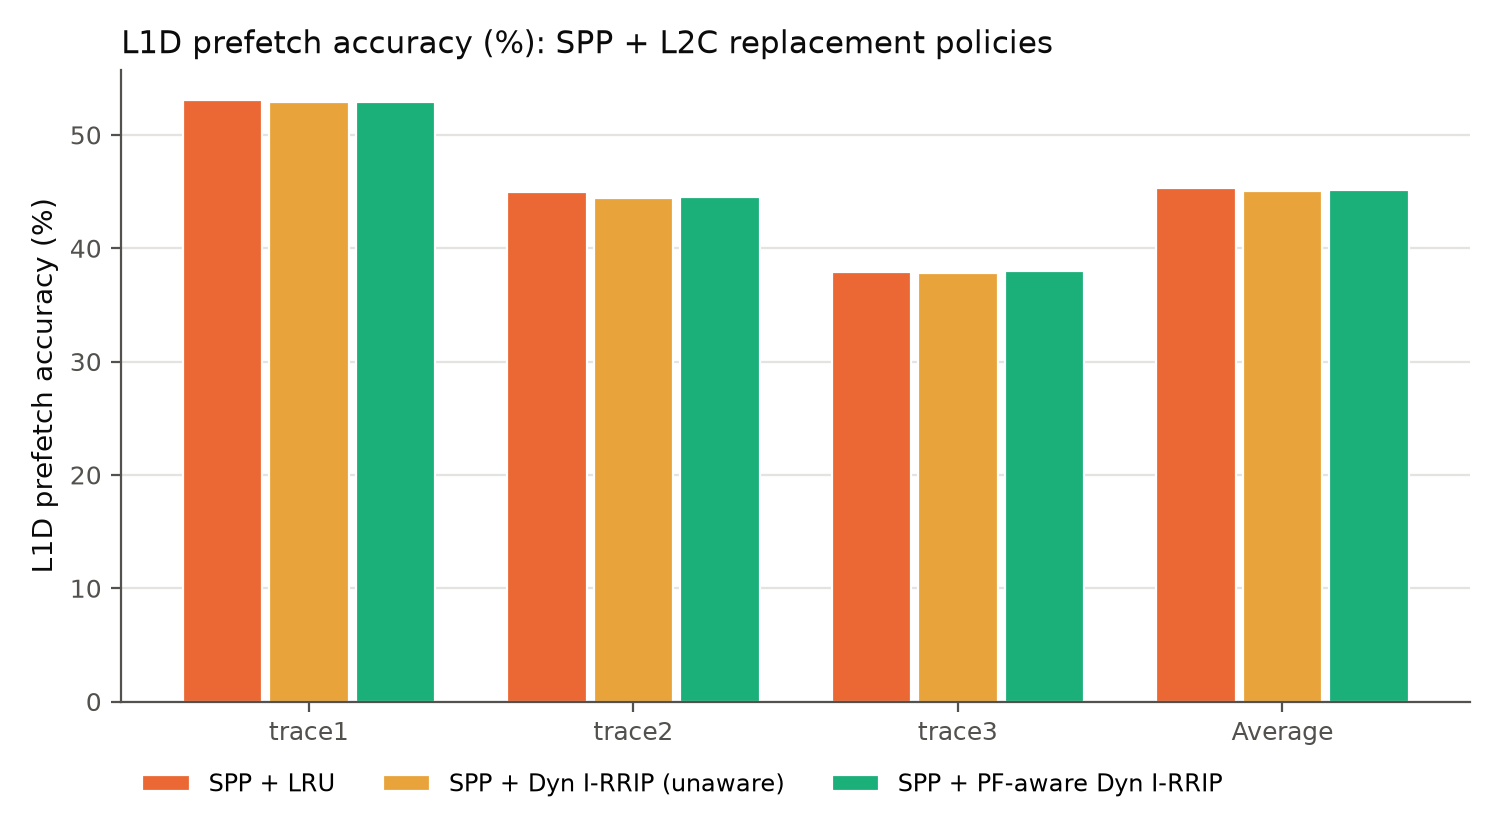
\includegraphics[width=\linewidth]{accuracy.png}\caption{L1D prefetch accuracy.}\end{subfigure}
\begin{subfigure}{0.49\textwidth}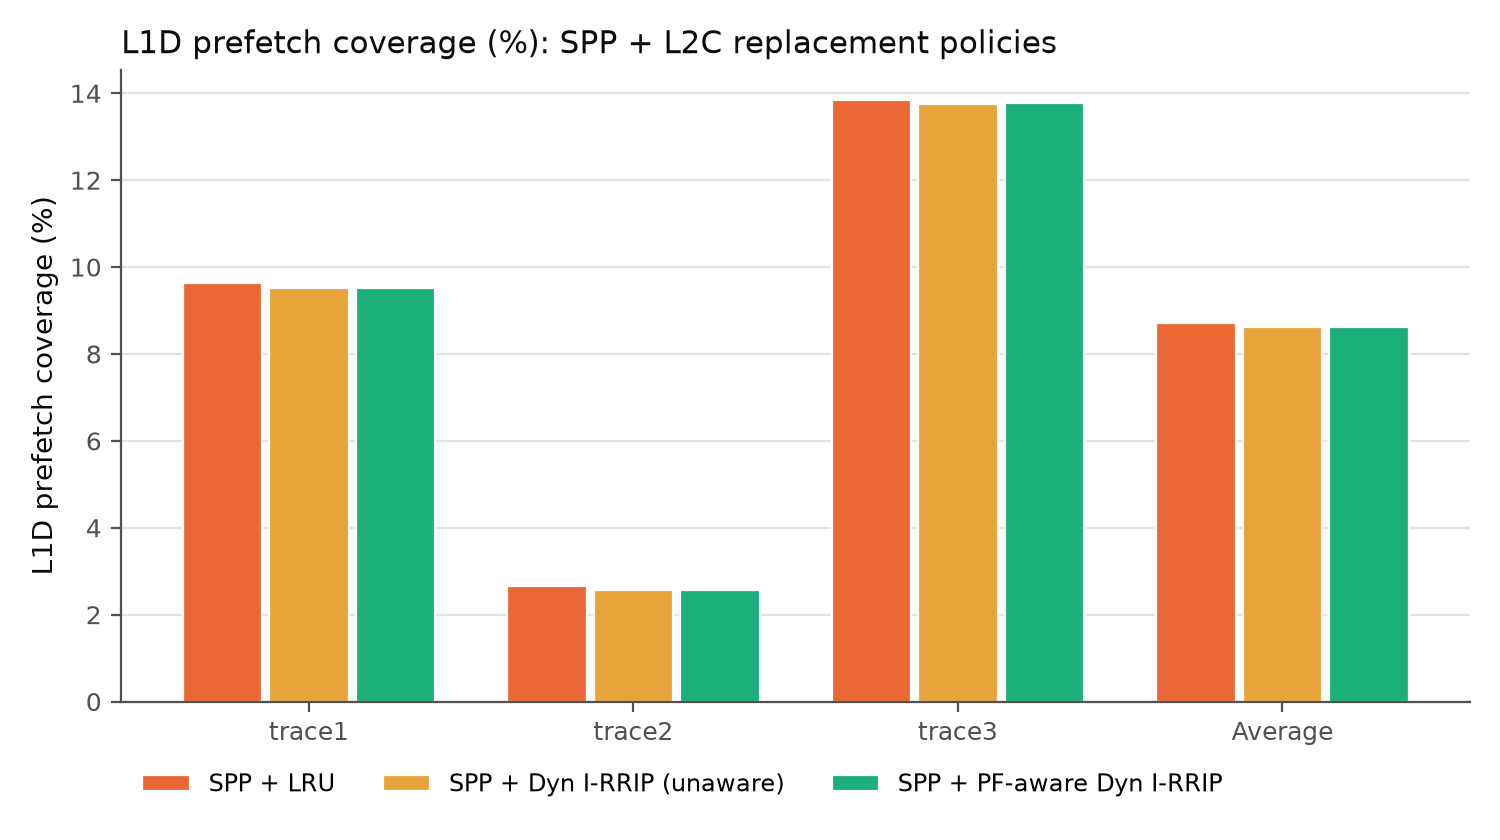
\includegraphics[width=\linewidth]{coverage.png}\caption{L1D prefetch coverage.}\end{subfigure}
\begin{subfigure}{0.49\textwidth}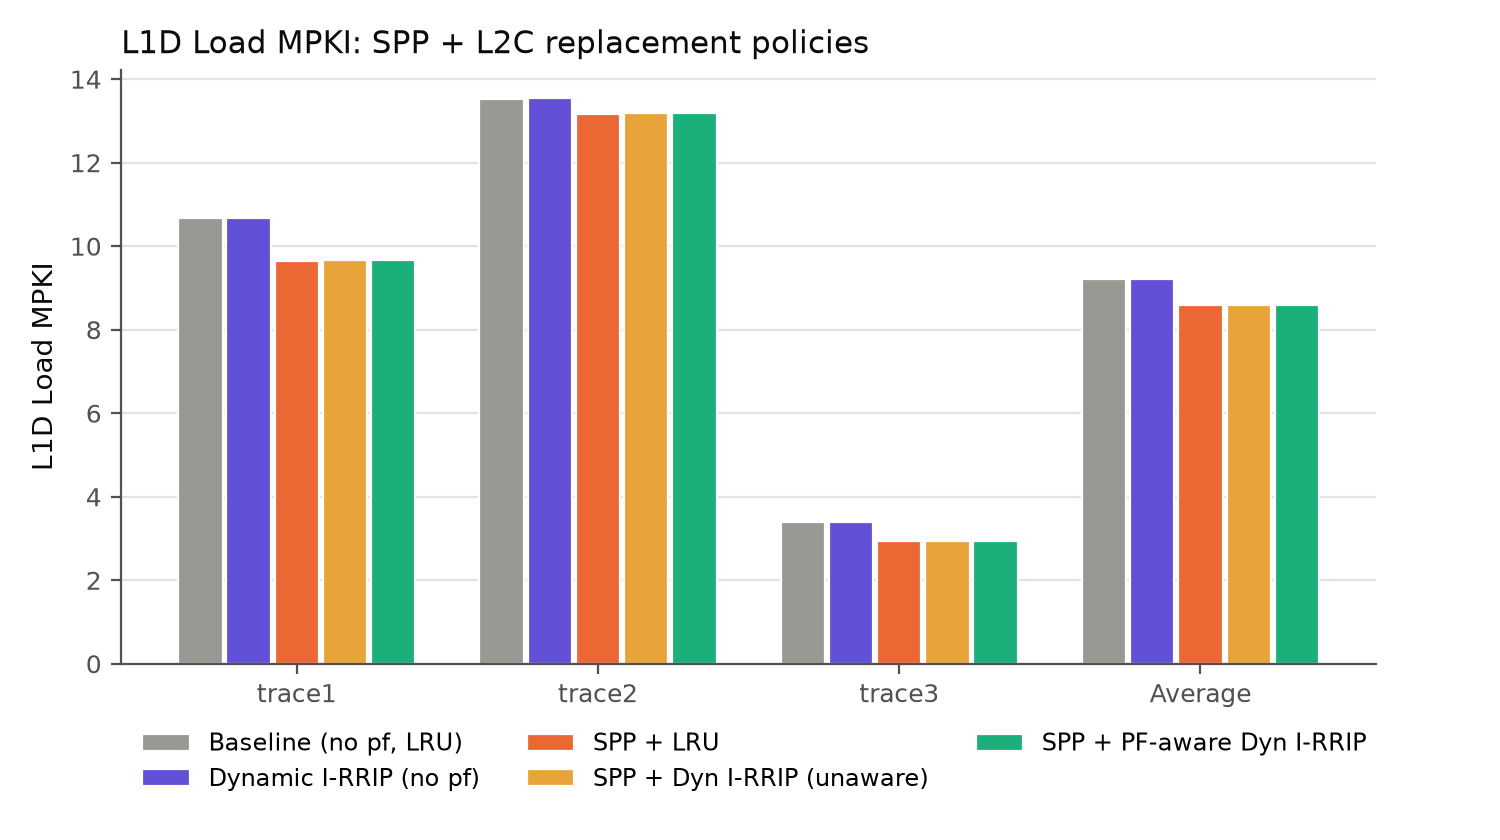
\includegraphics[width=\linewidth]{l1d_mpki.png}\caption{L1D load MPKI.}\end{subfigure}
\caption{L1D prefetch metrics. The L2 policy hardly changes SPP's accuracy and coverage.}
\label{fig:l1d}
\end{figure}

\begin{figure}[H]
\centering
\begin{subfigure}{0.49\textwidth}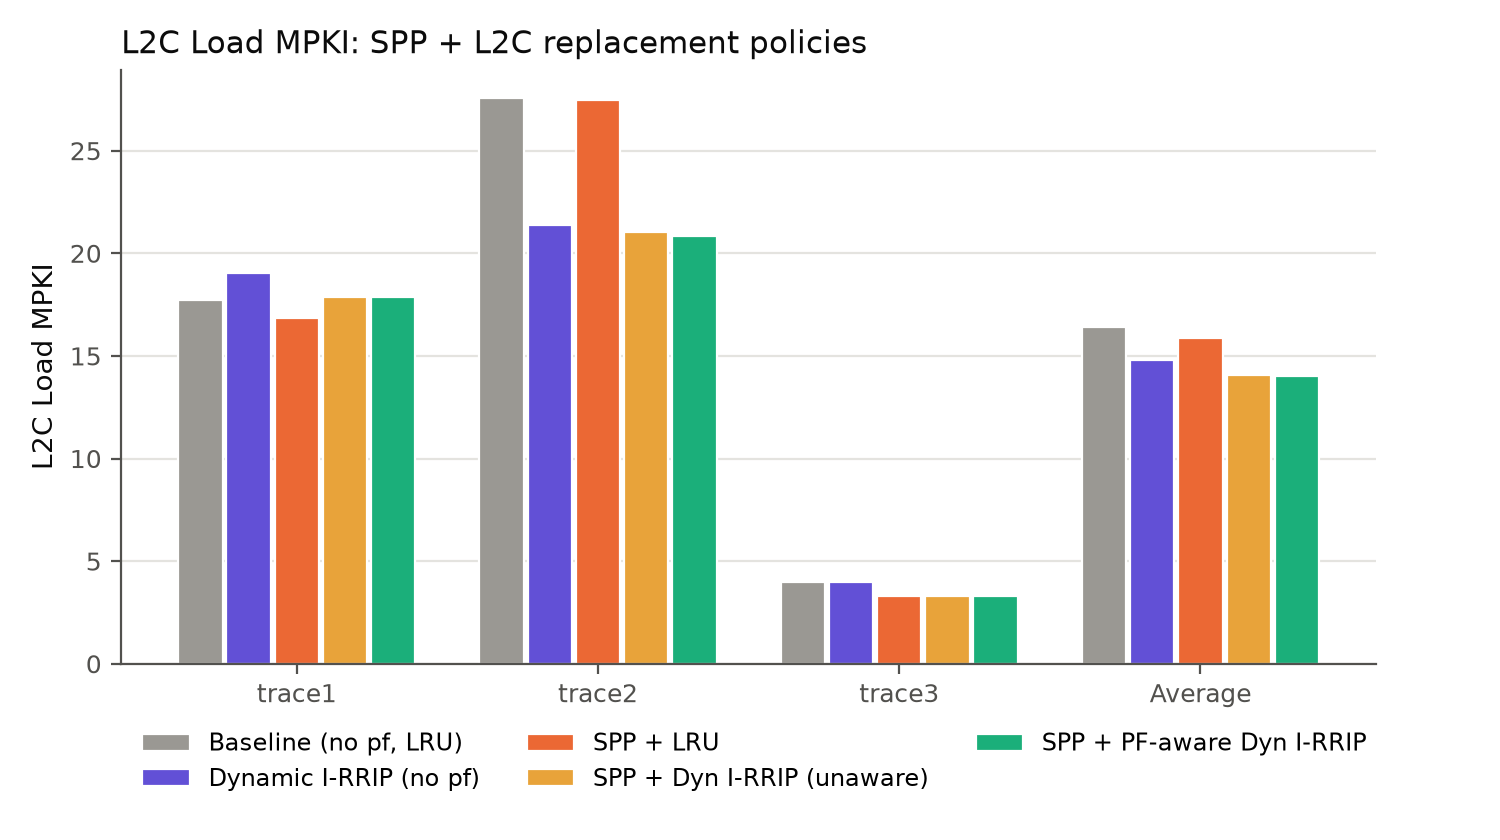
\includegraphics[width=\linewidth]{l2c_mpki.png}\caption{L2C load MPKI.}\end{subfigure}
\begin{subfigure}{0.49\textwidth}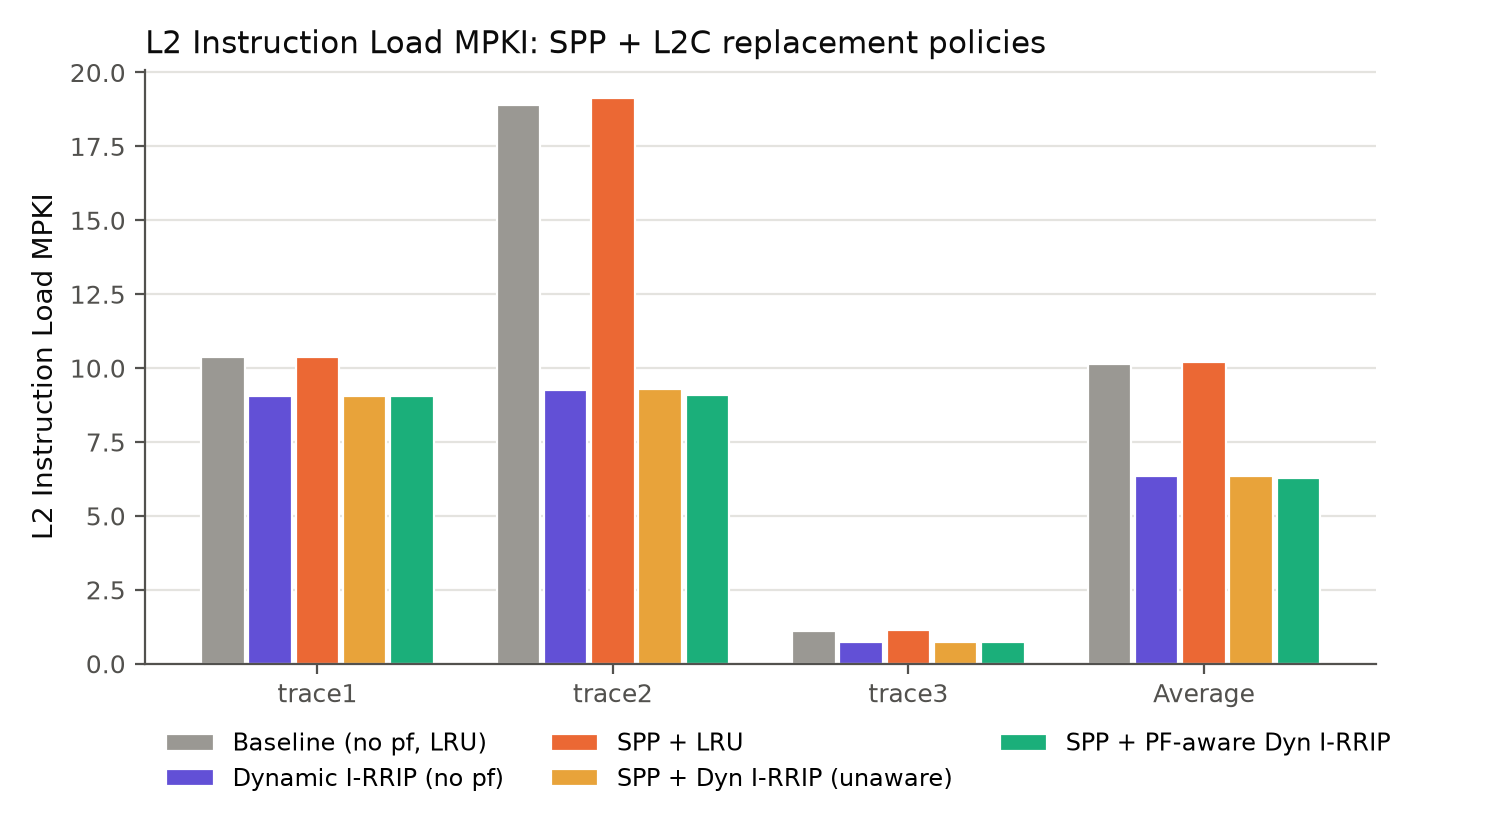
\includegraphics[width=\linewidth]{l2c_instr_mpki.png}\caption{L2 instruction load MPKI.}\end{subfigure}
\begin{subfigure}{0.49\textwidth}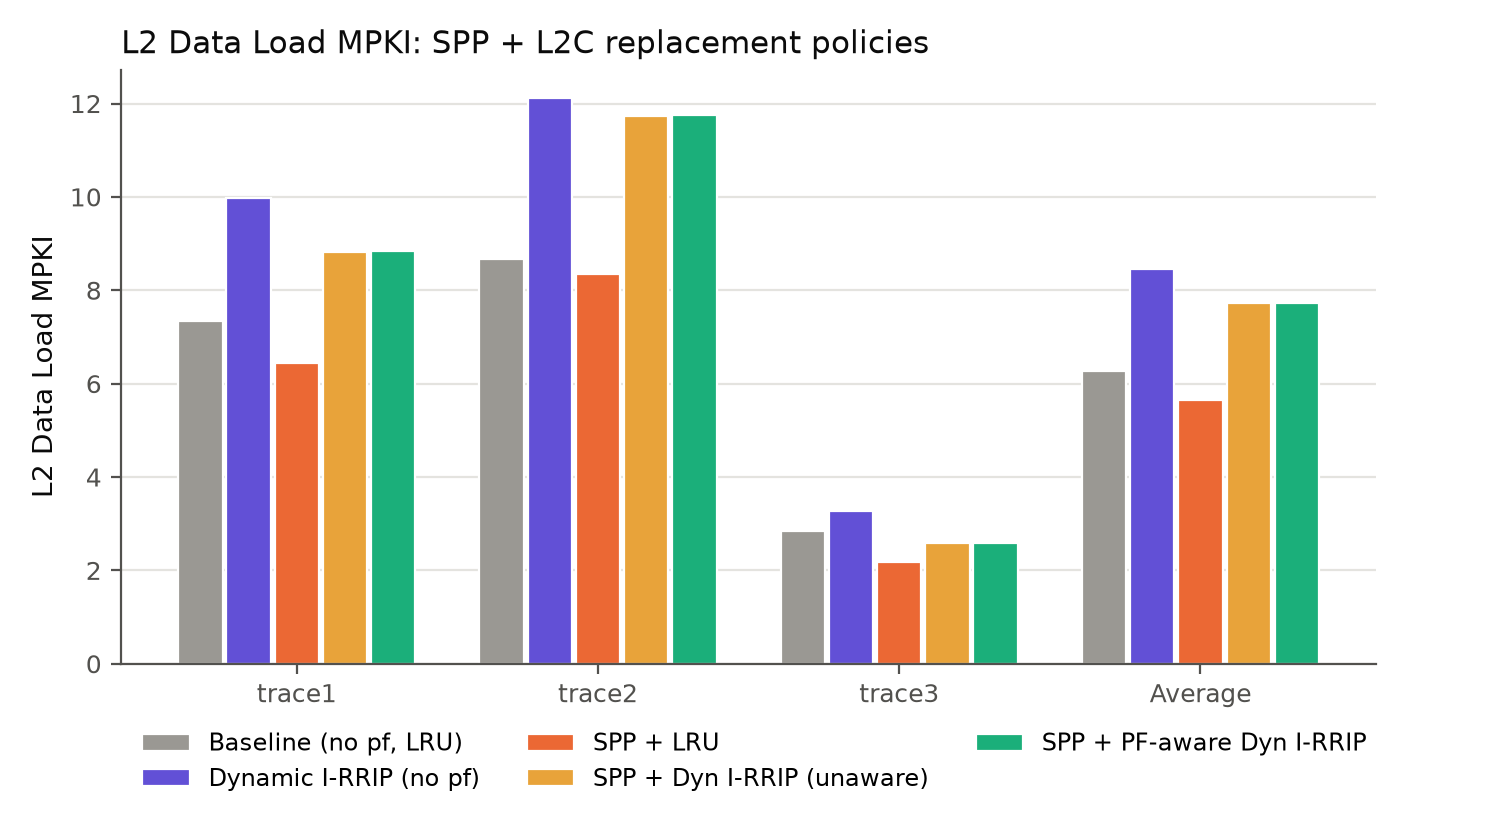
\includegraphics[width=\linewidth]{l2c_data_mpki.png}\caption{L2 data load MPKI.}\end{subfigure}
\caption{L2 load MPKI, in total and split by line type.}
\label{fig:l2}
\end{figure}

\subsection{Sensitivity study}
\label{sec:sens}

{\sloppy Both parameters of the final design are read from environment variables, namely
\texttt{DYN\_IRRIP\_PF\_INS} and \texttt{DYN\_IRRIP\_THRESHOLD}, so one binary covers
every point. Table~\ref{tab:sens} and Figure~\ref{fig:sens} vary one parameter at a time, keeping the
other at its final value.\par}

\begin{table}[H]
\centering
\small
\begin{adjustbox}{max width=\textwidth}
\begin{tabular}{lrrrrrrr}
\toprule
Value & Trace1 & Trace2 & Trace3 & Geomean & L2C load & L2 instr & L2 data \\
 & & & & speedup & MPKI & MPKI & MPKI \\
\midrule
\multicolumn{8}{l}{\emph{Prefetch fill insertion RRPV ($T = 0.05$)}}\\
0 & 1.0226 & 1.0442 & 1.0231 & 1.0299 & 14.014 & 6.295 & 7.718 \\
\textbf{1 (final)} & 1.0226 & 1.0445 & 1.0232 & \textbf{1.0301} & 14.010 & 6.288 & 7.722 \\
2 (= unaware) & 1.0222 & 1.0430 & 1.0229 & 1.0293 & 14.074 & 6.356 & 7.718 \\
3 & 1.0198 & 1.0430 & 1.0226 & 1.0284 & 14.078 & 6.361 & 7.717 \\
\midrule
\multicolumn{8}{l}{\emph{Leader-set threshold $T$ (prefetch insertion RRPV 1)}}\\
\textbf{0.05 (final)} & 1.0226 & 1.0445 & 1.0232 & \textbf{1.0301} & 14.010 & 6.288 & 7.722 \\
0.10 & 1.0226 & 1.0441 & 1.0227 & 1.0297 & 14.012 & 6.291 & 7.721 \\
0.20 & 1.0220 & 1.0395 & 1.0211 & 1.0275 & 14.032 & 6.418 & 7.613 \\
0.35 & 1.0217 & 1.0383 & 1.0169 & 1.0256 & 14.132 & 6.558 & 7.574 \\
0.50 & 1.0090 & 1.0366 & 1.0146 & 1.0200 & 13.843 & 7.124 & 6.719 \\
\bottomrule
\end{tabular}
\end{adjustbox}
\caption{Sensitivity of SPP + prefetch-aware Dynamic I-RRIP. Speedup over the baseline;
MPKI columns are means over the three traces. Insertion RRPV 2 with normal promotion is the
unaware policy, so that row matches the unaware configuration exactly.}
\label{tab:sens}
\end{table}

\begin{figure}[H]
\centering
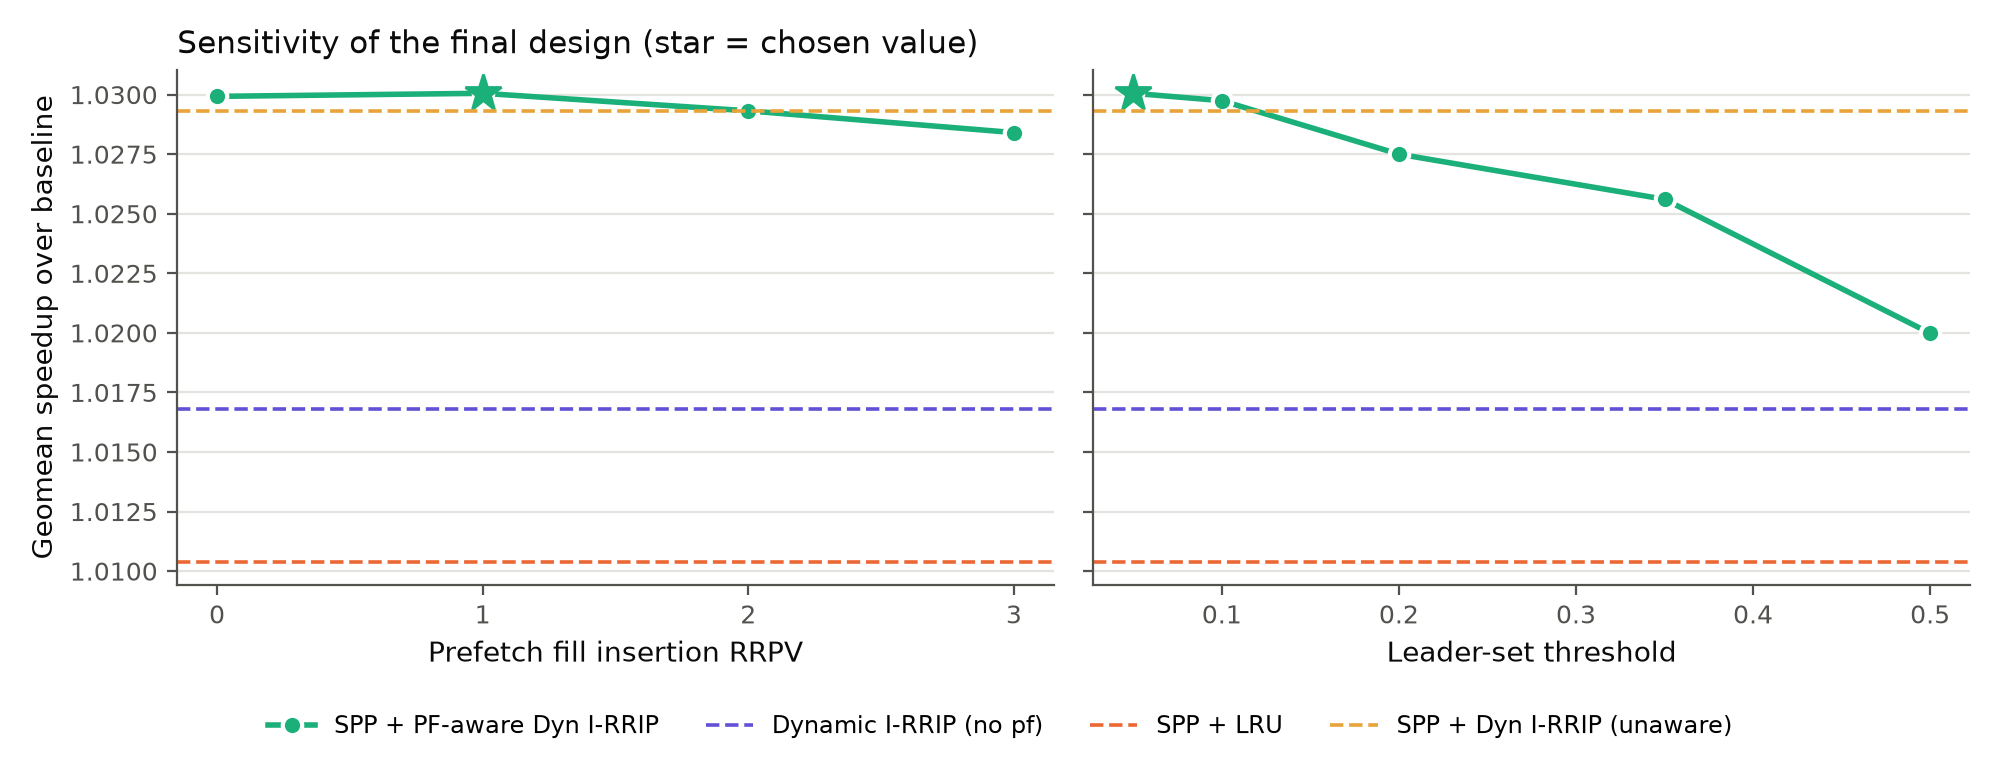
\includegraphics[width=\linewidth]{sensitivity.png}
\caption{Geomean speedup of the final design against the prefetch insertion RRPV (left) and the
leader-set threshold (right). The dashed lines are the other configurations.}
\label{fig:sens}
\end{figure}

\paragraph{Prefetch insertion.} The speedup rises monotonically as prefetched lines are given more
protection, from RRPV~3 to RRPV~1, and then falls slightly at RRPV~0. RRPV~0 ranks prefetched
data equal to code in instruction mode, and the L2 instruction MPKI starts to rise again (6.288
$\to$ 6.295). The gain of RRPV~1 over the unaware policy (RRPV~2) shows mainly on Trace2:
+0.14\%, with a lower total L2 load MPKI (21.04 $\to$ 20.84). On Trace2 this comes from fewer
instruction misses (9.30 $\to$ 9.10 MPKI); the data MPKI is unchanged. We did not isolate why a
different treatment of data prefetches lowers instruction misses; presumably it is a second-order
effect of the changed eviction order.

\paragraph{Threshold.} The Task 2B conclusion still holds with SPP. The speedup falls
monotonically as $T$ grows, and $T=0.05$ is the best value (or tied for best) on every trace. At $T=0.50$, Trace1
($r \approx 0.43$) spends 89\% of its epochs in SRRIP mode and loses most of its gain (1.0226
$\to$ 1.0090). Trace3 ($r \approx 0.17$) spends 33--67\% of its epochs in SRRIP from $T=0.20$
upwards. At the chosen $T=0.05$, all three traces stay in instruction mode for the whole measured
region.

\subsection{Analysis}

\paragraph{The goal is met on every trace.} SPP + prefetch-aware Dynamic I-RRIP has the highest IPC
on all three traces. The geometric-mean speedup is 1.0301: $+1.31\%$ over Dynamic I-RRIP alone
(1.0168) and $+1.95\%$ over standalone SPP (1.0104). Per trace, it is $+1.2\%$, $+0.9\%$ and
$+1.7\%$ over Dynamic I-RRIP, and $+1.4\%$, $+3.8\%$ and $+0.7\%$ over SPP.

\paragraph{The two mechanisms are complementary.} The product of the two individual speedups is
$1.0168 \times 1.0104 = 1.0274$, and the combination reaches 1.0293 even without awareness, so the
benefits add up rather than overlap. They remove different misses:
\begin{itemize}
  \item SPP removes L1D data misses (coverage 2.6--13.8\%) and does not change the L2 instruction
        MPKI.
  \item Dynamic I-RRIP cuts the L2 instruction MPKI by 38\% on average (10.22 $\to$ 6.29 with SPP).
        It does this at the cost of L2 data misses (5.65 $\to$ 7.72 MPKI with SPP).
  \item SPP softens that cost. With SPP, the L2 data MPKI under Dynamic I-RRIP is 7.72, compared
        with 8.45 without a prefetcher. That reduction (0.73) is slightly larger than what SPP
        achieves under LRU (6.28 $\to$ 5.65).
\end{itemize}
The L2 miss latency stays at Dynamic I-RRIP's low level, 101.7 cycles against 129.8 for SPP +
LRU. LLC load misses (DRAM trips) are the lowest of all configurations on Trace1 and Trace3.

\paragraph{The prefetch awareness adds a small but consistent gain.} Compared with SPP plus the
unaware Task 2B policy, the prefetch-aware policy is faster on every trace: Trace1 +0.04\%,
Trace2 +0.14\%, Trace3 +0.03\%, geomean 1.0293 $\to$ 1.0301. It also has fewer LLC load misses
on every trace, and lower total L2C and instruction MPKI on average. The gain is small for the
reason found in Section~\ref{sec:traffic}: SPP sends only 1.1--2.6 prefetches per kilo-instruction
to the L2, and 98\% of their L2 copies are never demanded there. No rule for those lines can
change much. The sensitivity and exploration results show that the \emph{direction} of the rule
matters more than its size. A policy that guesses wrongly in either direction is clearly worse
than the unaware one: dead-on-arrival insertion loses 0.09\%, and pinning prefetches loses
0.56\%.

\paragraph{SPP's accuracy and coverage are almost independent of the L2 policy.} Accuracy and
coverage change by at most 0.6 and 0.1 percentage points between the three SPP configurations
(Table~\ref{tab:main}). SPP trains on L1D accesses and throttles on its own L1D accuracy, so the
L2 policy changes when a prefetch completes (L2 hit or LLC access), not which lines are
prefetched. The speedup of the combined design therefore comes from the L2 side, as intended.

\subsection{Design exploration}
\label{sec:explore}

Before fixing the design, we evaluated a range of prefetch-handling options on all three traces
with an exploration build of the policy, in which every option sits behind an environment
variable (Table~\ref{tab:explore}).

\begin{table}[H]
\centering
\small
\begin{adjustbox}{max width=\textwidth}
\begin{tabular}{lrrrr}
\toprule
Prefetch handling (SPP + Dyn I-RRIP, $T=0.05$) & Trace1 & Trace2 & Trace3 & Geomean \\
\midrule
Unaware (Task 2B policy) & 1.0222 & 1.0430 & 1.0229 & 1.0293 \\
Fill RRPV 3, prefetch hit not promoted & 1.0196 & 1.0429 & 1.0225 & 1.0283 \\
Fill RRPV 3, prefetch hit promoted & 1.0198 & 1.0430 & 1.0226 & 1.0284 \\
Fill RRPV 2, prefetch hit not promoted & 1.0219 & 1.0430 & 1.0229 & 1.0292 \\
Fill RRPV 2, unused prefetches at RRPV 3 evicted first & 1.0218 & 1.0428 & 1.0228 & 1.0291 \\
Adaptive: RRPV 2/3 by L2 usefulness of recent prefetch fills & 1.0199 & 1.0429 & 1.0226 & 1.0284 \\
Fill RRPV 1, prefetch hit not promoted & 1.0220 & 1.0443 & 1.0232 & 1.0298 \\
\quad with leader sets ignoring prefetches & 1.0218 & 1.0444 & 1.0232 & 1.0297 \\
\textbf{Fill RRPV 1, prefetch hit promoted (final)} & 1.0226 & 1.0445 & 1.0232 & \textbf{1.0301} \\
\quad adaptive: RRPV 3 when recent L1D accuracy $<$ 40\% & 1.0225 & 1.0443 & 1.0228 & 1.0298 \\
\quad unused prefetches never evicted while other data exists & 1.0132 & 1.0402 & 1.0173 & 1.0235 \\
Fill RRPV 0, prefetch hit not promoted & 1.0227 & 1.0444 & 1.0229 & 1.0299 \\
Fill RRPV 0, prefetch hit promoted & 1.0226 & 1.0442 & 1.0231 & 1.0299 \\
\bottomrule
\end{tabular}
\end{adjustbox}
\caption{Prefetch-handling variants, as speedup over the baseline. Raw numbers, the legend and
all logs are in \texttt{results/task3/design\_exploration/}. The final design was also re-run
with a rebuilt binary, and the results were identical.}
\label{tab:explore}
\end{table}

\paragraph{Adaptive insertion did not pay off.} A natural idea is to set the insertion depth from
the measured usefulness of prefetches. Measured at the L2 (prefetched lines that get a demand hit
in the L2), the usefulness is only 1--2\% (Table~\ref{tab:traffic}) and never reached the 25\% threshold
in any epoch, so the adaptive policy always picks RRPV~3 and behaves like dead-on-arrival insertion. Measured at the L1D (SPP's own
accuracy, 38--53\% on average), the per-epoch accuracy hovers around a 40\% threshold: it is
above it in 86\%, 42\% and 39\% of the epochs on Trace1--3. The policy then alternates between
RRPV~1 and RRPV~3 and lands between the two fixed policies (1.0298). On these traces neither signal separates good phases from bad
ones, so a fixed insertion depth is enough. Adaptive insertion would matter for a prefetcher whose accuracy swings between
phases. SPP already throttles its own degree by accuracy (Task 1B), which reduces the need for it.

\paragraph{Writebacks.} For completeness we also tried inserting writeback fills at RRPV~3. Dynamic
I-RRIP turns many L1D writebacks into L2 misses (68.9\% writeback miss rate on Trace2, against
3.0\% for SPP + LRU), most likely because data lines are evicted first in instruction
mode. This lowered the
speedup to 1.0286, so writebacks keep the Task 2B treatment. It is not part of the prefetch
handling.

\subsection{Limitations}

The prefetch-aware rules add only $+0.08\%$ geomean on top of the plain combination, because
little prefetch traffic reaches the L2 with this L1D prefetcher. The rules would matter more for
an L2 prefetcher or a more aggressive L1D prefetcher, but we could not evaluate those within the
assignment's configuration. The insertion RRPV and the threshold were chosen on the same three
traces they are evaluated on, so the measured gains may be optimistic for unseen workloads. The
small instruction-MPKI improvement on Trace2 from prefetch-aware insertion was observed but not
explained mechanistically.

\subsection{Reproducing the results}
\begin{verbatim}
./build_champsim.sh no  lru       baseline
./build_champsim.sh no  dyn_irrip dyn_irrip
./build_champsim.sh spp lru       spp
./build_champsim.sh spp dyn_irrip spp_dyn_irrip
# the provided traces are gzip files without an extension
mkdir -p traces
for i in 1 2 3; do ln -sf ../Trace$i-00$i traces/trace$i.champsimtrace.gz; done
task3/run_task3.sh traces 12     # 3 traces x (5 configs + 7 sensitivity)
python3 task3/parse_results.py  # task3_tables.md, task3_results.csv
python3 task3/plot_results.py   # results/task3/plots/
# single run; DYN_IRRIP_PF_AWARE=0 gives the unaware
# Task 2B behaviour, DYN_IRRIP_PF_INS sets the RRPV
DYN_IRRIP_PF_INS=1 bin/<spp_dyn_irrip binary> \
    -warmup_instructions 25000000 \
    -simulation_instructions 25000000 \
    -traces traces/trace1.champsimtrace.gz
\end{verbatim}

\end{document}
